%
% File: chap01.tex
% Author: Victor F. Brena-Medina
% Description: Introduction chapter where the biology goes.
%
\let\textcircled=\pgftextcircled
\chapter{Programmability of the FPGA}
\label{chap:programmability_design}
\paragraph{}

\section{Overview}

\paragraph{}
In the previous chapter, the I/O Block was designed in Cadence Schematic L. This chapter will focus on the programmability of the FPGA. We first discuss the configuration bits used across the FPGA, then carefully size the configuration 6-T cell to avoid unintended bit flips. Finally, we design the row and column decoders in Cadence Schematic L. 

\section{Configuration memory architecture}
\paragraph{}

Each CLB requires 32 configuration bits which are organized into two 4X4 SRAM arrays. Each center switch matrix requires 16 configuration bits laid in a 4X4 SRAM array. Each edge switch matrix requires 12 configuration bits laid out in a 4X3 SRAM array. Lastly, each I/O block requires 16 configuration bits laid in a 4X4 SRAM array. All the memory bits have been carefully organised into arrays of column width 4. This allows us to program the FPGA 4 bits at a time. These 4 bits may be supplied parallely or can be internally buffered from a faster single bit stream. We see that increasing this programming parallelism beyond 4 doesn't scale elegantly. Furthermore, programming more bits at a time increases the current and power consumption of the chip in configuration phase. This is why, we limit us to 4 bits at a time. Also, this only affects the speed with which the FPGA can be programmed and does not affect the FPGA performance at all.

\section{Sizing a memory cell}
\paragraph{}

The architecture we are using has common wordlines and bitlines. So, we have to take care of the fact that when you are not driving a bitline, its capacitive charge shouldn't change the memory contents even if it's worldline is raised. This situation occurs when you are trying to write neighbouring 4-bits sharing the same wordline. This was taken care of while minimally sizing the 6-T cell (see Fig. 6.1). We used a 5X safety over the bitline capacitance reported by a captab analysis using spectre in ADE L. This is to account for the RC parasitics of the wires in the layout of the FPGA.

\begin{figure}[H]
\centering
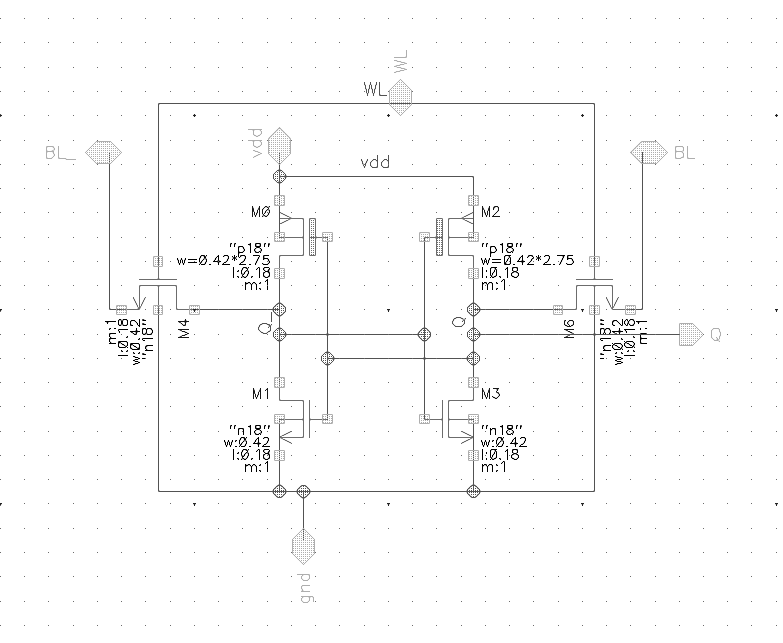
\includegraphics[width=0.9\textwidth]{6tcell.png}
\caption{6-T SRAM cell Schematic}
\label{fig:Figure}
\end{figure}

\begin{figure}[H]
\centering
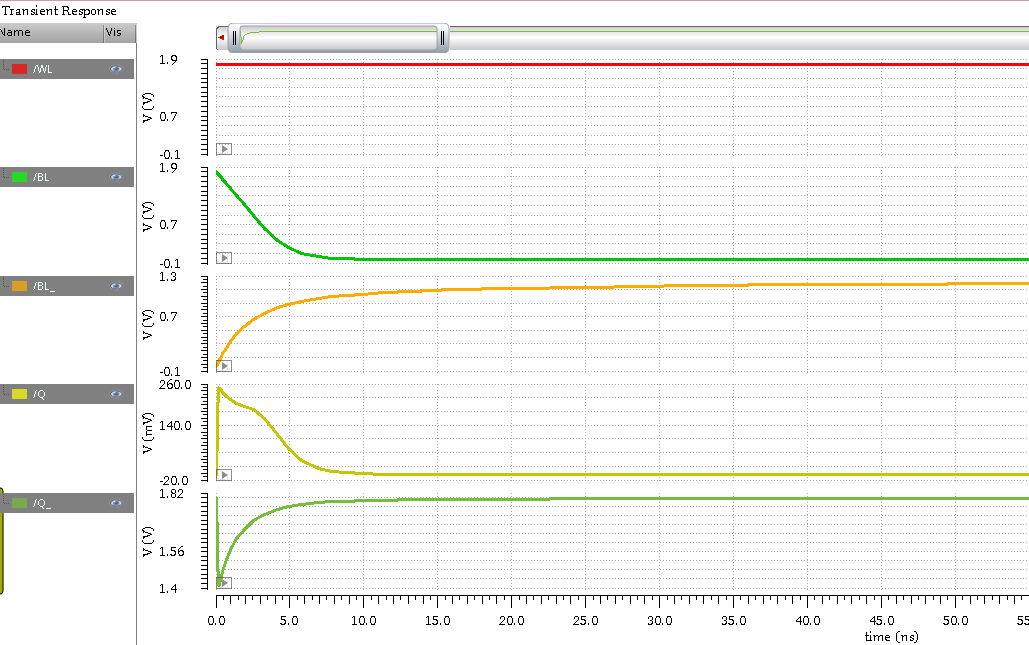
\includegraphics[width=\textwidth]{6trecovery.png}
\caption{6-T cell parasitic flip recovery}
\label{fig:Figure}
\end{figure}
The simulation in Fig. 6.2 shows that when the bitlines are in a state opposite to the memory data at the time when wordline is raised, the cell corrects the stray value on the bitline capacitances with the actual data values instead of getting corrupted.
\section{Designing the row decoder}
\paragraph{}
We use SKILL language by Candence to automatically generate the schematic from a text file.

\section{Designing the column decoder}
\paragraph{}
We use SKILL language by Candence to automatically generate the schematic from a text file. The generated schematics of row and column decoders are shown in Fig. 6.3.

\begin{figure}[h]
\begin{subfigure}{0.5\linewidth}
\centering
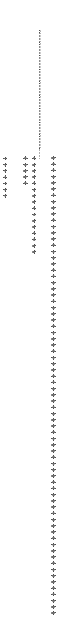
\includegraphics[]{rowdecoder_schematic.png}
\caption{row decoder}
\label{fig:Figure}
\end{subfigure}
\begin{subfigure}{0.5\linewidth}
\centering
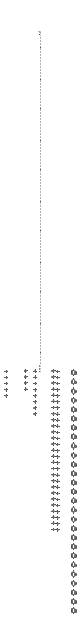
\includegraphics[]{columndecoder_schematic.png}
\caption{column decoder}
\label{fig:Figure}
\end{subfigure}
\caption{Schematics of row and column decoder}
\label{fig:Figure}
\end{figure}

\section{Hot-swapping and partial reconfiguration}
\paragraph{}
Since the read circuitory of LUTs uses decoders to read the truth table at any given time, it is independent of the write circuitory of the LUTs. Similar argument can be made for the configuration bits in the CLBs, switch matrices and I/O blocks. Therefore, the FPGA can be partially reconfigured on the fly. Also, the truth tables can be hot-swapped to change the functionality on the fly. This functionality comes inherently with our FPGA architecture.

\section{Summary}
\paragraph{}
This chapter describes the programmability of the FPGA. The whole 8X8 FPGA uses 74 wordlines and 108 bitlines. 7 bits are used for row address decoding and 5 bits are used for decoding the 27(108/4) column addresses.


